\section{Generated Worlds}
With the following command we can generate some examples of the model we 
formalized.
\lstinputlisting[language=alloy, firstline=134, lastline=139]{alloy/model.als}
In particular we are asking the solver to have in our sample world at least 2
\emph{Operators}, 2 \emph{Users}, 2 \emph{Locations} and 2 \emph{Violations}.
Furthermore we are limiting the maximum cardinality for each entity at 4, and
the Integers in our model have a bitwidth of 9.

The output of the Alloy Analyzer for the previous command is the following:
\begin{lstlisting}
Executing "Run show for 4 but 9 int"
    Solver=sat4j Bitwidth=9 MaxSeq=4 SkolemDepth=1 Symmetry=20
    108896 vars. 4360 primary vars. 376105 clauses. 574ms.
    Instance found. Predicate is consistent. 1736ms.
\end{lstlisting}
and it shows that all the facts are consistent. The world generated with the
previous command is shown in figure \vref{fig:alloy_world}.

\begin{figure}[hb]
    \centering
    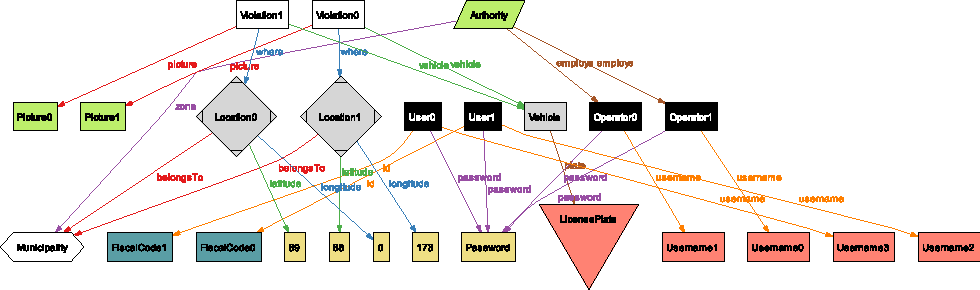
\includegraphics[width=\textwidth]{alloy_world}
    \caption{World generated from the Alloy model}
    \label{fig:alloy_world}
\end{figure}